% BP-SGT architecture figure (paper style).
% Drawn from SparseGT_BP/sgt/sgt_decoder.py (SparseGTBPDecoder.refine / forward / decode)
% and Nvidia_GNN+BP(lLatest)/common/bp.py (staged_decode), final config of SparseGT_BP/README.md:
% S = 4 SGT stages, T = 10 or 40 BP iterations, BP restarted each stage, k = ceil(0.5 n),
% 2 pre-LN blocks, d = 64, h = 4 heads, FFN 128, global attention + Tanner-graph pair bias,
% |L| selection, residual fix on the previous prior.
% Build: see README.md (pdflatex, then pdftocairo for PNG / SVG).
\documentclass[tikz,border=6pt]{standalone}
\usepackage{amsmath,amssymb,bm}
\usetikzlibrary{positioning,arrows.meta,fit,backgrounds,calc}

% ---------- palette (one colour per module family) ----------
\definecolor{bpC}{HTML}{4C72B0}
\definecolor{sgtC}{HTML}{DD8452}
\definecolor{statC}{HTML}{B8941F}
\definecolor{selC}{HTML}{C44E52}
\definecolor{biasC}{HTML}{8172B3}
\definecolor{tfC}{HTML}{55A868}
\definecolor{headC}{HTML}{3A9E9A}
\definecolor{okC}{HTML}{3D8B4F}
\definecolor{inkC}{HTML}{2B2B2B}

\tikzset{
  >={Stealth[length=2.2mm,width=1.6mm]},
  every node/.style={font=\small, text=inkC},
  blk/.style={draw=#1, fill=#1!13, line width=0.8pt, rounded corners=3pt, align=center,
              minimum height=1.25cm, inner sep=2pt},
  sm/.style={draw=#1, fill=#1!13, line width=0.7pt, rounded corners=2pt, align=center,
             minimum height=0.55cm, inner sep=2pt, font=\footnotesize},
  flow/.style={->, line width=0.8pt, draw=inkC},
  tsh/.style={font=\scriptsize, text=inkC!85, inner sep=1pt},
  sub/.style={font=\scriptsize, text=inkC!80},
  panel/.style={font=\normalsize\bfseries, anchor=west},
  ptitle/.style={font=\small\itshape, anchor=west},
  op/.style={circle, draw=inkC, line width=0.7pt, fill=white, inner sep=0pt, minimum size=4.4mm, font=\footnotesize},
  vn/.style={circle, draw=inkC, line width=0.6pt, fill=white, minimum size=3.6mm, inner sep=0pt},
  cn/.style={rectangle, draw=inkC, line width=0.6pt, fill=white, minimum size=3.2mm, inner sep=0pt},
}

\begin{document}
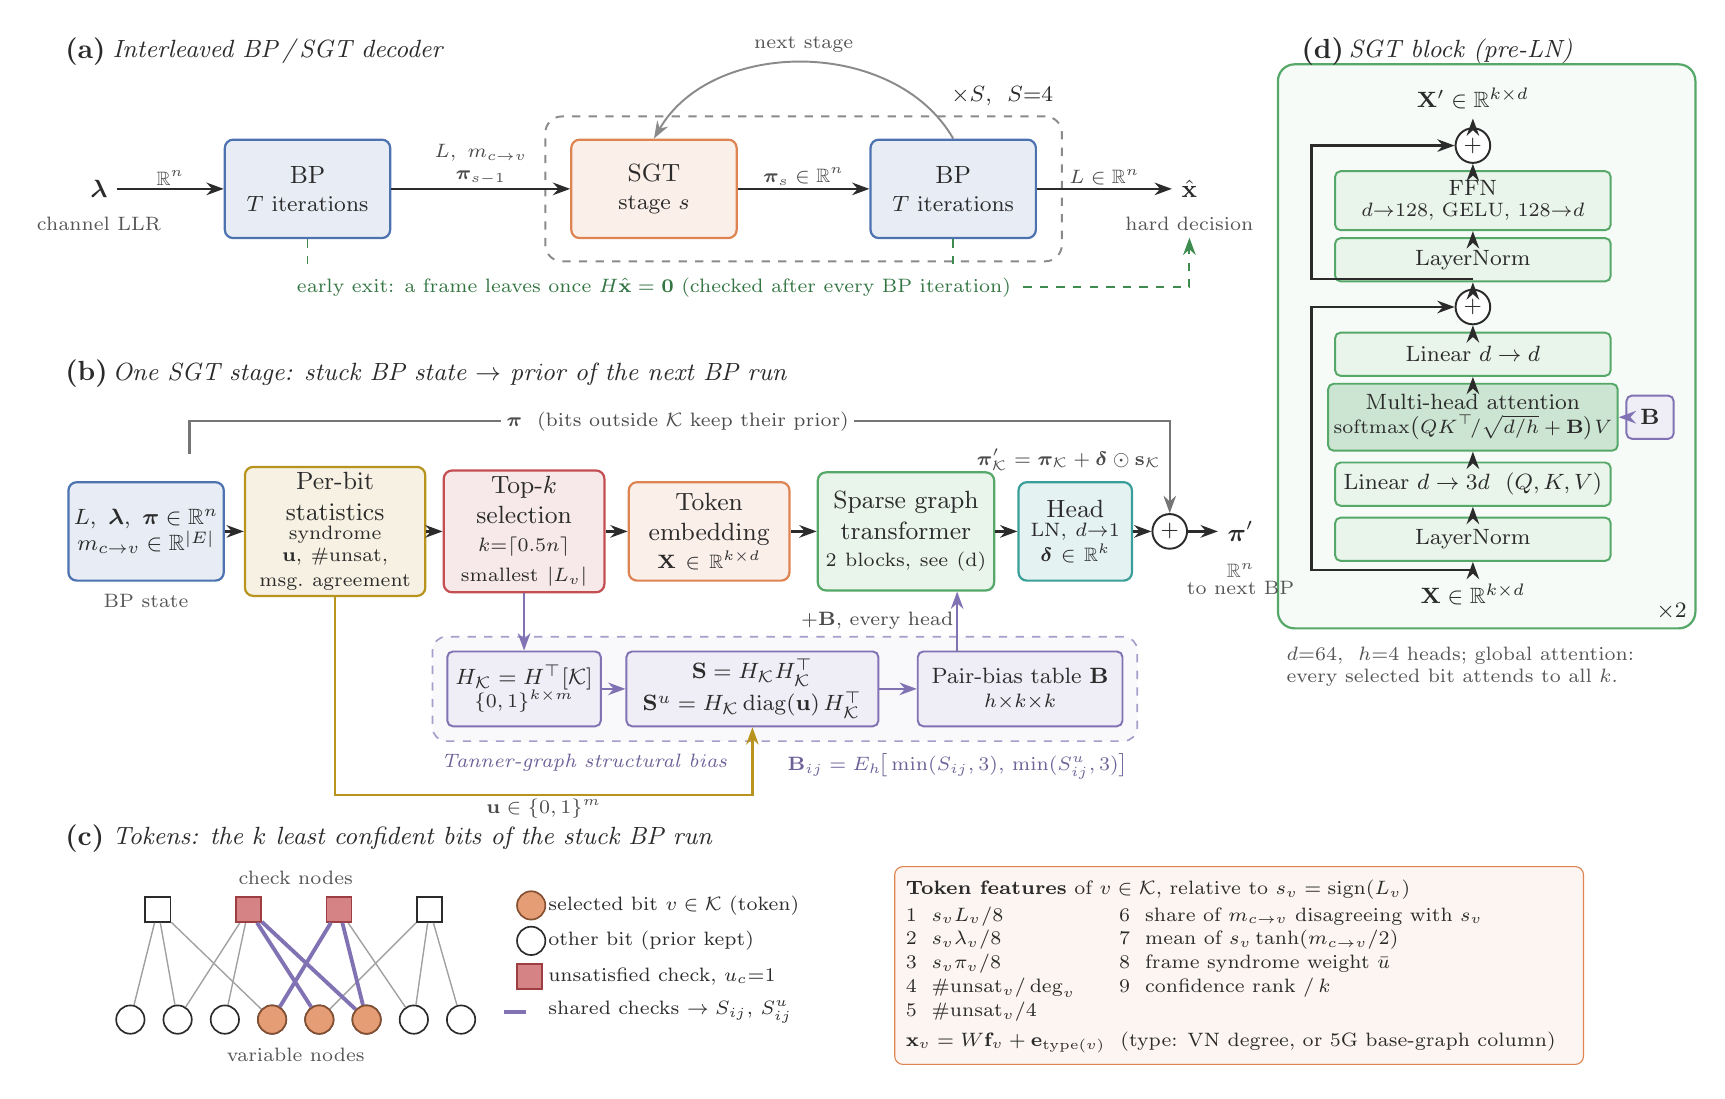
\begin{tikzpicture}

% =====================================================================
% (a) Interleaved pipeline
% =====================================================================
\node[panel] at (-0.3, 1.75) {(a)};
\node[ptitle] at (0.3, 1.75) {Interleaved BP\,/\,SGT decoder};

\node (y)   at (0.25,0) {$\bm{\lambda}$};
\node[sub, align=center, below=0pt of y] {channel LLR};
\node[blk=bpC,  minimum width=2.1cm] (bp0) at (2.9,0)  {BP\\[-1pt]{\footnotesize $T$ iterations}};
\node[blk=sgtC, minimum width=2.1cm] (sgt) at (7.3,0)  {SGT\\[-1pt]{\footnotesize stage $s$}};
\node[blk=bpC,  minimum width=2.1cm] (bp1) at (11.1,0) {BP\\[-1pt]{\footnotesize $T$ iterations}};
\node (xh)  at (14.1,0) {$\hat{\mathbf{x}}$};
\node[sub, align=center, below=0pt of xh] {hard decision};

\draw[flow] (y) -- node[tsh, above] {$\mathbb{R}^{n}$} (bp0);
\draw[flow] (bp0) -- node[tsh, above, align=center] {$L,\ m_{c\to v}$\\$\bm{\pi}_{s-1}$} (sgt);
\draw[flow] (sgt) -- node[tsh, above] {$\bm{\pi}_{s}\in\mathbb{R}^{n}$} (bp1);
\draw[flow] (bp1) -- node[tsh, above] {$L\in\mathbb{R}^{n}$} (xh);

\begin{scope}[on background layer]
  \node[draw=inkC!55, dashed, line width=0.7pt, rounded corners=6pt, fit=(sgt)(bp1), inner xsep=9pt, inner ysep=8pt] (rep) {};
\end{scope}
\node[anchor=south east, font=\footnotesize] at (rep.north east) {$\times S$, \ $S{=}4$};
\draw[->, line width=0.7pt, draw=inkC!55] (bp1.north) to[out=120,in=60] node[sub, above] {next stage} (sgt.north);

% early-exit rail
\coordinate (rail) at (0, -1.25);
\draw[okC, line width=0.7pt, dashed, ->] (bp0.south) -- (bp0.south |- rail) -- (xh |- rail) -- ($(xh)+(0,-0.62)$);
\draw[okC, line width=0.7pt, dashed] (bp1.south) -- (bp1.south |- rail);
\fill[okC] (bp0.south |- rail) circle (1.4pt) (bp1.south |- rail) circle (1.4pt);
\node[font=\scriptsize, text=okC!85!black, fill=white, inner sep=2pt] at (7.3,-1.25)
  {early exit: a frame leaves once $H\hat{\mathbf{x}}=\mathbf{0}$ (checked after every BP iteration)};


% =====================================================================
% (b) One SGT stage
% =====================================================================
\node[panel] at (-0.3, -2.35) {(b)};
\node[ptitle] at (0.3, -2.35) {One SGT stage: stuck BP state $\rightarrow$ prior of the next BP run};

\def\ym{-4.35}
\node[draw=bpC, fill=bpC!13, line width=0.8pt, rounded corners=3pt, align=center, font=\footnotesize,
      minimum width=1.75cm, minimum height=1.25cm, inner sep=2pt] (in) at (0.85,\ym)
      {$L,\ \bm{\lambda},\ \bm{\pi}\in\mathbb{R}^{n}$\\$m_{c\to v}\in\mathbb{R}^{|E|}$};
\node[sub, below=1pt of in] (inlab) {BP state};
\node[blk=statC, minimum width=2.1cm, text width=2.15cm] (stat) at (3.25,\ym)
  {Per-bit\\statistics\\[-1pt]{\scriptsize syndrome $\mathbf{u}$, \#unsat,\\[-2pt]msg.\ agreement}};
\node[blk=selC, minimum width=1.95cm, text width=1.9cm] (sel) at (5.65,\ym)
  {Top-$k$\\selection\\[-1pt]{\scriptsize $k{=}\lceil 0.5n\rceil$ smallest $|L_v|$}};
\node[blk=sgtC, minimum width=1.95cm, text width=1.9cm] (emb) at (8.0,\ym)
  {Token\\embedding\\[-1pt]{\scriptsize $\mathbf{X}\in\mathbb{R}^{k\times d}$}};
\node[blk=tfC, minimum width=2.15cm, text width=2.1cm, minimum height=1.5cm] (tf) at (10.5,\ym)
  {Sparse graph\\transformer\\[-1pt]{\scriptsize $2$ blocks, see (d)}};
\node[blk=headC, minimum width=1.35cm, text width=1.3cm] (head) at (12.65,\ym)
  {Head\\[-1pt]{\scriptsize LN, $d{\to}1$\\[-2pt]$\bm{\delta}\in\mathbb{R}^{k}$}};
\node[op] (plus) at (13.85,\ym) {$+$};
\node (pout) at (14.75,\ym) {$\bm{\pi}'$};

\draw[flow] (in) -- (stat);
\draw[flow] (stat) -- (sel);
\draw[flow] (sel) -- (emb);
\draw[flow] (emb) -- (tf);
\draw[flow] (tf) -- (head);
\draw[flow] (head) -- (plus);
\draw[flow] (plus) -- (pout);

\node[sub, below=1pt of pout, align=center] {$\mathbb{R}^{n}$\\[-2pt]to next BP};

% residual prior path
\draw[flow, draw=inkC!65] (in.north) ++(0.55,0.35) |- (13.85,-2.95) -- (plus.north);
\node[tsh, fill=white, inner sep=2pt] at (7.6,-2.95) {$\bm{\pi}$ \ (bits outside $\mathcal{K}$ keep their prior)};
\node[tsh, anchor=south east] at (13.78,-3.62) {$\bm{\pi}'_{\mathcal{K}}=\bm{\pi}_{\mathcal{K}}+\bm{\delta}\odot\mathbf{s}_{\mathcal{K}}$};

% structural-bias branch
\def\yb{-6.35}
\node[sm=biasC, minimum width=1.95cm, minimum height=0.95cm] (Hk) at (5.65,\yb)
  {$H_{\mathcal{K}}=H^{\top}[\mathcal{K}]$\\[-1pt]{\scriptsize $\{0,1\}^{k\times m}$}};
\node[sm=biasC, minimum width=3.2cm, minimum height=0.95cm] (S) at (8.55,\yb)
  {$\mathbf{S}=H_{\mathcal{K}}H_{\mathcal{K}}^{\top}$\\[1pt]$\mathbf{S}^{u}=H_{\mathcal{K}}\,\mathrm{diag}(\mathbf{u})\,H_{\mathcal{K}}^{\top}$};
\node[sm=biasC, minimum width=2.6cm, minimum height=0.95cm] (B) at (11.95,\yb)
  {Pair-bias table $\mathbf{B}$\\[-1pt]{\scriptsize $h{\times}k{\times}k$}};
\draw[flow, draw=biasC] (sel) -- (Hk);
\draw[flow, draw=biasC] (Hk) -- (S);
\draw[flow, draw=biasC] (S) -- (B);
\draw[flow, draw=biasC] (11.15,0 |- B.north) -- node[tsh, left] {$+\mathbf{B}$, every head} (11.15,0 |- tf.south);
\draw[flow, draw=statC] (stat.south) -- (stat.south |- 0,-7.7) -| node[tsh, pos=0.25, below] {$\mathbf{u}\in\{0,1\}^{m}$} (S.south);
\begin{scope}[on background layer]
  \node[draw=biasC!70, fill=biasC!5, rounded corners=5pt, dashed, line width=0.6pt, fit=(Hk)(S)(B), inner sep=5pt] (biasbox) {};
\end{scope}
\node[anchor=north west, font=\scriptsize\itshape, text=biasC!85!black] at ($(biasbox.south west)+(0,-0.03)$)
  {Tanner-graph structural bias};
\node[anchor=north east, font=\scriptsize, text=biasC!85!black] at ($(biasbox.south east)+(0,-0.03)$)
  {$\mathbf{B}_{ij}=E_h\!\big[\min(S_{ij},3),\,\min(S^{u}_{ij},3)\big]$};

% =====================================================================
% (c) selection on the Tanner graph + token features
% =====================================================================
\def\yc{-8.25}
\node[panel] at (-0.3, \yc) {(c)};
\node[ptitle] at (0.3, \yc) {Tokens: the $k$ least confident bits of the stuck BP run};

\foreach \i in {1,...,8} { \node[vn] (v\i) at ({0.6*\i+0.05}, \yc-2.3) {}; }
\foreach \j/\x in {1/1.0,2/2.15,3/3.3,4/4.45} { \node[cn] (c\j) at (\x, \yc-0.9) {}; }
\foreach \j/\list in {1/{1,2,4},2/{2,3,5,6},3/{4,6,7},4/{5,7,8}} {
  \foreach \i in \list { \draw[line width=0.5pt, draw=inkC!45] (c\j) -- (v\i); } }
\foreach \j in {2,3} { \node[cn, fill=selC!70, draw=selC!80!black] at (c\j) {}; }
\draw[line width=1.4pt, draw=biasC] (c2) -- (v5) (c2) -- (v6) (c3) -- (v4) (c3) -- (v6);
\foreach \i in {4,5,6} { \node[vn, fill=sgtC!80, draw=sgtC!60!black] at (v\i) {}; }
\node[sub] at (2.75, \yc-2.75) {variable nodes};
\node[sub] at (2.75, \yc-0.5) {check nodes};

\begin{scope}[shift={(5.55,\yc-0.85)}, every node/.style={font=\scriptsize, anchor=west, text=inkC, inner sep=2pt}]
  \node[vn, fill=sgtC!80, draw=sgtC!60!black] at (0,0) {}; \node at (0.33,0) {selected bit $v\in\mathcal{K}$ (token)};
  \node[vn] at (0,-0.45) {}; \node at (0.33,-0.45) {other bit (prior kept)};
  \node[cn, fill=selC!70, draw=selC!80!black] at (0,-0.9) {}; \node at (0.33,-0.9) {unsatisfied check, $u_c{=}1$};
  \draw[line width=1.4pt, draw=biasC] (-0.15,-1.35) -- (0.13,-1.35); \node at (0.33,-1.35) {shared checks $\rightarrow S_{ij},\,S^{u}_{ij}$};
\end{scope}

\node[anchor=north west, font=\scriptsize, draw=sgtC, fill=sgtC!8, rounded corners=3pt, inner sep=4pt] at (10.35,\yc-0.35) {%
\renewcommand{\arraystretch}{1.08}%
\begin{tabular}{@{}r@{\ \ }l@{\qquad}r@{\ \ }l@{}}
\multicolumn{4}{@{}l}{\textbf{Token features} of $v\in\mathcal{K}$, relative to $s_v=\mathrm{sign}(L_v)$}\\[1pt]
1 & $s_v L_v/8$          & 6 & share of $m_{c\to v}$ disagreeing with $s_v$\\
2 & $s_v \lambda_v/8$    & 7 & mean of $s_v\tanh(m_{c\to v}/2)$\\
3 & $s_v \pi_v/8$        & 8 & frame syndrome weight $\bar{u}$\\
4 & \#unsat$_v/\deg_v$  & 9 & confidence rank $/\,k$\\
5 & \#unsat$_v/4$       &   & \\[2pt]
\multicolumn{4}{@{}l}{$\mathbf{x}_v=W\mathbf{f}_v+\mathbf{e}_{\mathrm{type}(v)}$ \ (type: VN degree, or 5G base-graph column)}\\
\end{tabular}};

% =====================================================================
% (d) SGT block inset
% =====================================================================
\def\xd{17.7}
\node[panel] at (15.4, 1.75) {(d)};
\node[ptitle] at (16.0, 1.75) {SGT block (pre-LN)};
\begin{scope}[every node/.style={font=\footnotesize, text=inkC}]
  \node (dout) at (\xd, 1.15) {$\mathbf{X}'\in\mathbb{R}^{k\times d}$};
  \node[op] (r2) at (\xd, 0.55) {$+$};
  \node[sm=tfC, minimum width=3.5cm, minimum height=0.75cm] (ff) at (\xd, -0.15) {FFN\\[-2pt]{\scriptsize $d{\to}128$, GELU, $128{\to}d$}};
  \node[sm=tfC, minimum width=3.5cm] (ln2) at (\xd, -0.90) {LayerNorm};
  \node[op] (r1) at (\xd, -1.50) {$+$};
  \node[sm=tfC, minimum width=3.5cm] (proj) at (\xd, -2.10) {Linear $d\to d$};
  \node[sm=tfC, minimum width=3.5cm, fill=tfC!30, minimum height=0.85cm] (att) at (\xd, -2.90) {Multi-head attention\\[-1pt]{\scriptsize $\mathrm{softmax}\big(QK^{\top}\!/\sqrt{d/h}+\mathbf{B}\big)V$}};
  \node[sm=tfC, minimum width=3.5cm] (qkv) at (\xd, -3.75) {Linear $d\to3d$ \ ($Q,K,V$)};
  \node[sm=tfC, minimum width=3.5cm] (ln1) at (\xd, -4.45) {LayerNorm};
  \node (din) at (\xd, -5.15) {$\mathbf{X}\in\mathbb{R}^{k\times d}$};
\end{scope}
\draw[flow] (din) -- (ln1); \draw[flow] (ln1) -- (qkv); \draw[flow] (qkv) -- (att);
\draw[flow] (att) -- (proj); \draw[flow] (proj) -- (r1); \draw[flow] (r1) -- (ln2);
\draw[flow] (ln2) -- (ff); \draw[flow] (ff) -- (r2); \draw[flow] (r2) -- (dout);
\draw[flow] ($(din.north)+(0,0.05)$) -- ++(-2.05,0) |- (r1);
\draw[flow] ($(r1.north)+(0,0.12)$) -- ++(-2.05,0) |- (r2);
\node[sm=biasC, minimum width=0.6cm] (bin) at (\xd+2.25, -2.90) {$\mathbf{B}$};
\draw[flow, draw=biasC] (bin) -- (att);
\coordinate (dl) at (\xd-2.3, -5.15);
\coordinate (dr) at (\xd+2.65, 1.15);
\begin{scope}[on background layer]
  \node[draw=tfC, fill=tfC!5, rounded corners=6pt, line width=0.8pt, fit=(din)(dout)(dl)(dr), inner sep=5pt] (dbox) {};
\end{scope}
\node[anchor=south east, font=\footnotesize] at (dbox.south east) {$\times 2$};
\node[anchor=north west, sub, align=left] at ($(dbox.south west)+(0,-0.1)$)
  {$d{=}64$, \ $h{=}4$ heads; global attention:\\every selected bit attends to all $k$.};

\end{tikzpicture}
\end{document}
